\documentclass[letterpaper]{article}

% --- Packages
\usepackage[utf8]{inputenc}
\usepackage[T1]{fontenc}
\usepackage[margin=0.25cm]{geometry}
\usepackage{enumitem}
\usepackage{pdfpages}
\usepackage{multicol}
\usepackage{amsmath}
\usepackage{amssymb}
\usepackage[skip=1pt plus1pt, indent=0pt]{parskip}
\usepackage{enumitem}
\usepackage{graphicx}

% --- Data
\title{Electrical field and potential}
\author{Enrique Calderon}
\date{March 2024}

% --- Graphics path
\graphicspath{ {./img/} }

% --- Custom commands
\makeatletter
\let\thetitle\@title
\let\theauthor\@author
\makeatother
\newcommand{\compconj}[1]{%
    \overline{#1}%
}
\newcommand{\divline}{\noindent\makebox[\linewidth]{\rule{\textwidth}{0.4pt}}}
\newcommand{\taninv}{\tan^{-1}}
 
% Example of image adding
%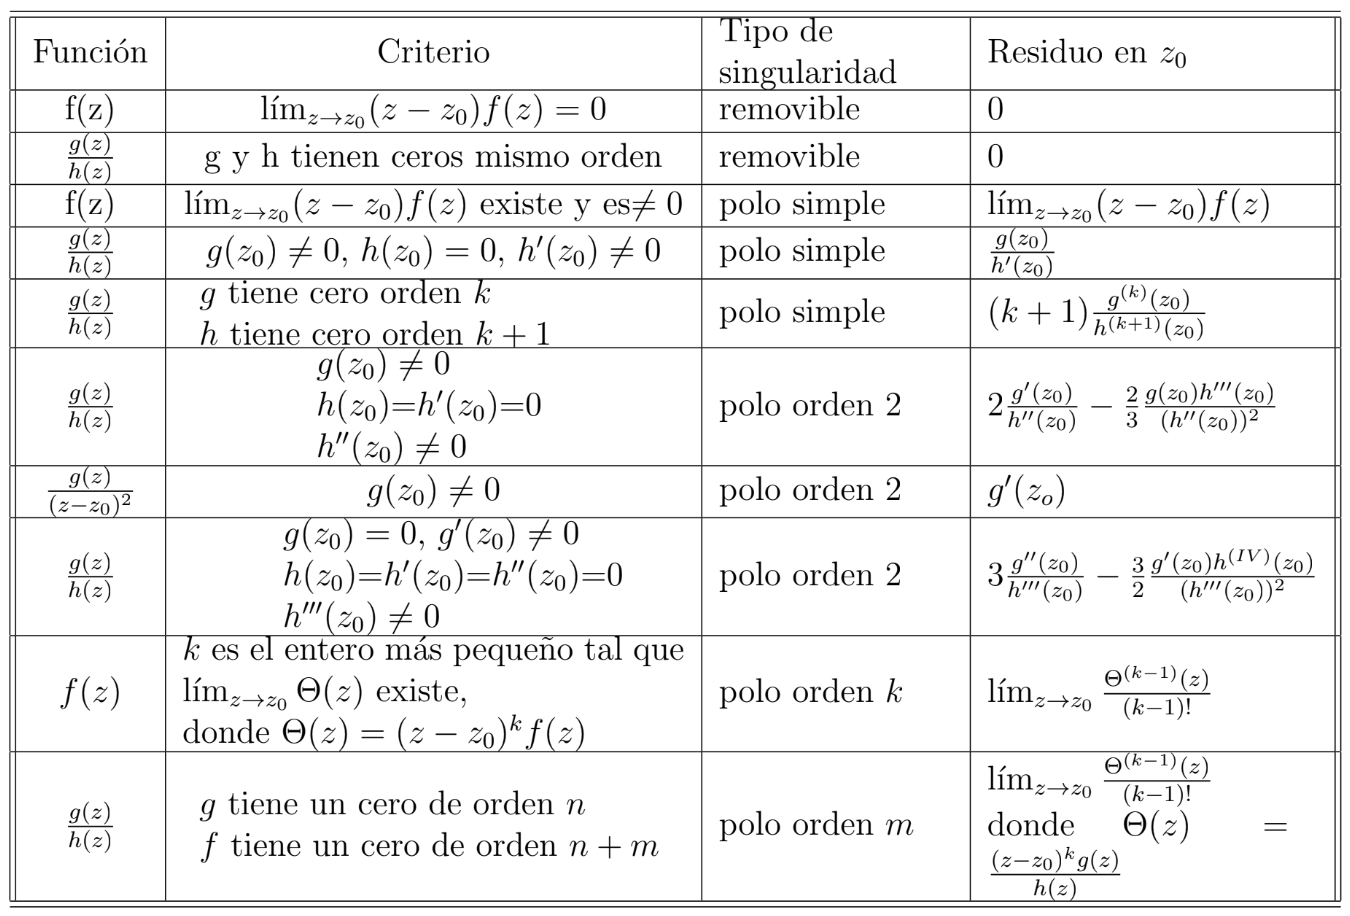
\includegraphics[width=0.8\textwidth]{ResidueTable}

% Remember to add divline between sections

\begin{document}
    \maketitle

    \divline
    \begin{multicols}{2}
        \section{Electric charge and distributions}
        
        Linear electric charge density:
        
        \[\lambda = \frac{Q}{l} \left[\frac{C}{m}\right]\]

        Superficial electric charge density:

        \[\sigma = \frac{Q}{A} \left[\frac{C}{m^{2}}\right]\]

        Q : Total electric charge
    \end{multicols}

    \divline
    \begin{multicols}{2}
        \section{Coulomb law. Electric force in vector form}
        
        Electric force:

        \[F = k \frac{|q_{1}||q_{2}|}{r^{2}}[N]\]

        \[k = \frac{1}{4 \pi \epsilon} \left[\frac{N \cdot m^{2}}{C^{2}}\right] \]

        \(\epsilon_{0}\) : Permittivity of air \( 8.8542 \times 10^{-12} \left[\frac{C^{2}}{N \cdot m^{2}}\right] \)

        \(k\) : Coulomb's constant \(9 \times 10^{9} \left[\frac{N \cdot m^{2}}{C^{2}}\right] \)

        In vector form:

         \[\overline{F} = \left| \frac{1}{4 \pi \epsilon_{0}} \frac{|q_{1}||q_{2}|}{r^{2}} \right| \hat{u}  [N]\]
        
    \end{multicols}

    \divline
    \begin{multicols}{2}
        \section{Electric field as a vector field}
        
        Electric field:

        \[\overline{E} = \frac{\overline{F}_{q0}}{q_{0}} \left[ \frac{N}{C} \right] \]

        \begin{itemize}
            \item Positive charge has arrows outside and negative charge has arrows entering.
            \item Electric field vector in a point is tangent to the line.
            \item The number of lines is proportional to the value of electric charge.
        \end{itemize}
    \end{multicols}

    \divline
    \begin{multicols}{2}
        \section{Obtaining electric fields in vector form for discrete distributions}
        
        \subsection{Originated by a punctual charge}

        \[\overline{E_{A}} = k \frac{|q|}{r^{2}} \hat{u}  \left[ \frac{N}{C} \right] \]

        \subsection{Originated by a linear distribution}

        \[\overline{E_{P}} = k |\lambda| \int \frac{dl}{r^{2}} \hat{u} \left[ \frac{N}{C} \right] \]

        \subsection{Originated by a superficial distribution}

        \[ \overline{E_{P}} = k |\sigma| \iint \frac{dA}{r^{2}} \hat{u} \left[ \frac{N}{C} \right] \]

        \subsection{Originated by a infinite line}

        \[\overline{E_{P \lambda}} = \frac{2k|\lambda|}{a} \hat{u} \left[ \frac{N}{C} \right]\]

        \subsection{Originated by a ring}

        \[ \overline{E_{P}} =  \frac{kb|q|}{(b^{2}+R^{2})^{\frac{3}{2}}}  \hat{u} \left[ \frac{N}{C} \right] \]

        \subsection{Originated by a big or infinite surface}

        \[ \overline{E_{P}} = \frac{|\sigma|}{2\epsilon_{0}} \left( 1 - \frac{b}{(b^{2} + R^{2})^{\frac{1}{2}}} \right)  \hat{u} \left[ \frac{N}{C} \right] \]

        \[ \overline{E_{P}} = \frac{|\sigma|}{2\epsilon_{0}} \hat{u} \left[ \frac{N}{C} \right] \]

        Where \(a\) is the minimal distance between line and point.
    \end{multicols}

    \divline
    \begin{multicols}{2}
        \section{Electrical flow}
        In a open surface:

        \[\phi_{E} = \iint \overline{E} \cdot \hat{n} dA \left[ \frac{N \cdot m^{2}}{C} \right] \]

        If a surface is closed and the source of electric field is outside the electric flow is 0.

        In a closed surface:

        If a surface is closed and the source of electric field is outside the electric flow is 0.

        If the source is inside:

        \[\phi_{E} = \oint\oint \overline{E} \cdot \hat{n} dA \left[ \frac{N \cdot m^{2}}{C} \right] \]
    \end{multicols}

    \divline
    \begin{multicols}{2}
        \section{Gauss law}

        Defined as:
        
        \[\phi_{E} = \frac{Q_{\text{locked}}}{\epsilon_{0}} \left[ \frac{N \cdot m^{2}}{C} \right] \]

        And as a differential form:

        \[\overrightarrow{\nabla} \cdot \overrightarrow{E} = \frac{\rho}{\epsilon_{0}}\]

        Where \(\rho\) is the density of volumetric electrical charge.

        \subsection{Electric field originated from a sphere with electric charge}

        \[\overrightarrow{E_{p}} = \frac{1}{4 \pi \epsilon_{0}} \frac{|Q_{\text{esf}}|}{r^{2}} \hat{u} \left[ \frac{N}{C} \right] \]

        Where \(Q_{\text{esf}} = \rho_{\text{esf}}A_{\text{esf}}\)

        \subsection{Electric field originated from a infinite line}

        \[\overrightarrow{E_{p}} = \frac{2k |\lambda|}{a} \hat{u} \left[ \frac{N}{C} \right] \]

        \subsection{Electric field originated by a infinite surface}

        \[\overrightarrow{E_{p}} = \frac{|\rho|}{2\epsilon_{0}} \hat{u} \left[ \frac{N}{C} \right]\]
    \end{multicols}
    
    \divline
    \begin{multicols}{2}
        \section{Electrostatic field circulation and rotational}
        \[c = \oint \overline{E} \cdot d \overline{l} = 0\]

        \[rot \overline{E} = \overline{\nabla} \times \overline{E} = \overline{0}\]
    \end{multicols}

    \divline
    \begin{multicols}{2}
        \section{Electric potential energy}

        \[V_{a} = \frac{_{\infty} W_{A}}{q} \left[ \frac{J}{C} \right] = - \int_{\infty}^{A} \overline{E} \cdot d \overline{l} \left[ V \right] \]

        \[V_{AB} = - V_{BA}\]
    \end{multicols}

    \divline
    \begin{multicols}{2}
        \section{Potential differences}

        \subsection{Originated by a punctual charge}

        \[V_{AB} = kq \left( \frac{1}{r_{A}} - \frac{1}{r_{B}} \right) [V]\]

        \subsection{Originated by a infinite line}

        \[V_{AB} = 2k\lambda \left( \frac{r_{B}}{r_{A}} \right) [v]\]

        \subsection{Originated by a big surface}

        \[V_{AB} = \frac{\sigma}{2 \epsilon_{0}} (r_{B} - r_{A}) [V]\]
    \end{multicols}

    \divline
    \begin{multicols}{2}
        \section{Electric potential gradient}

        \[\overline{\nabla} V = \frac{\delta V}{\delta x} \hat{i} + \frac{\delta V}{\delta y} \hat{j} + \frac{\delta V}{\delta z} \hat{k} \left[ \frac{V}{m} \right] \]

        In other coordinates systems:

        \[\overline{\nabla} V = \frac{\delta V}{\delta r} \hat{r} + \frac{1}{r \sin{\phi}} \frac{\delta V}{\delta \theta} \hat{\theta} + \frac{1}{r} \frac{\delta V}{\delta \phi} \hat{\phi} \left[ \frac{V}{m} \right] \]

        \[\overline{\nabla} V = \frac{\delta V}{\delta r} \hat{r} + \frac{1}{r} \frac{\delta V}{\delta \theta} \hat{\theta} + \frac{\delta V}{\delta z} \hat{z} \left[ \frac{V}{m} \right] \]

        Electric field as the potential gradient

        \[\overline{E} =   - \overline{\nabla} V =  - \left( \frac{\delta V}{\delta x} \hat{i} + \frac{\delta V}{\delta y} \hat{j} + \frac{\delta V}{\delta z} \hat{k} \right) \left[ \frac{V}{m} \right] \]

        \[\overline{E} = \overline{E_{x}} + \overline{E_{y}} + \overline{E_{z}} \]
        
        
    \end{multicols}
    

\end{document}
